\documentclass[a4paper,12pt]{article}

% Including packages for common needs
\usepackage[utf8]{inputenc}
\usepackage[T1]{fontenc}
\usepackage{lmodern}
\usepackage{amsmath, amssymb}
\usepackage{geometry}
\geometry{a4paper, margin=0.8in}
\usepackage{graphicx}
\usepackage{hyperref}
\usepackage{caption}
\usepackage{subcaption}
\usepackage{booktabs}
\usepackage{array}
\usepackage{siunitx} % For percentages and numbers formatting
\usepackage{placeins}
\usepackage{pdflscape}
\usepackage{float}
\usepackage{enumitem}
\usepackage{titlesec}
\usepackage{titling}
\usepackage{geometry}
\geometry{a4paper, margin=0.8in}

% Setting up the document title and author
\title{Optimización del Modelo de Detección de Fraude minimizando Falsas Alarmas en Clientes Frecuentes}
\author{Adrian Rodríguez}
\date{29 de mayo de 2025}

\usepackage{titling}
\setlength{\droptitle}{-3em}
\pretitle{\begin{center}\Large\bfseries}
\posttitle{\par\end{center}\vskip 0.5em}
\preauthor{\begin{center}\normalsize}
\postauthor{\end{center}}
\predate{\begin{center}\small}
\postdate{\par\end{center}\vskip -1em}

\begin{document}

% Generating the title
\maketitle

% Section 1: Resumen Ejecutivo
\section{Resumen Ejecutivo}
El presente informe sintetiza las actividades de exploración, ingeniería de características, modelado y evaluación realizadas sobre un conjunto de \textbf{1 852 394 transacciones} (enero-2019 $\rightarrow$ diciembre-2020) con el fin de reducir las \textbf{falsas alarmas} (FP) en el segmento de \textbf{clientes frecuentes legítimos} sin sacrificar la capacidad de detección de fraude (recall).

Los hallazgos clave son:
\begin{itemize}
    \item \textbf{Clientes frecuentes} ($\geq$ 4 compras/mes en el mismo comercio) representan \textbf{\SI{1.4}{\percent}} de las transacciones y exhiben tasas de fraude sensiblemente menores al promedio.
    \item El \textbf{modelo base LightGBM} (AUC $\approx$ 0,993) logró un recall $\approx$ 0,79 con un \textbf{FP Rate global 0,057 \si{\percent}} y \textbf{FP Rate en clientes frecuentes 0,052 \si{\percent}} tras optimizar el umbral.
    \item Introducir \textbf{métricas personalizadas} –especialmente \texttt{business\_fp\_tp\_ratio}– y \textbf{pesos diferenciados} para transacciones legítimas de clientes frecuentes, seguido de \textbf{búsqueda bayesiana con Optuna}, produjo un \textbf{modelo optimizado} que:
    \begin{itemize}
        \item \textbf{Eliminó} los FP en clientes frecuentes (0 incidencias).
        \item \textbf{Redujo} los FP globales a \textbf{0,017 \si{\percent}} ($-$70 \si{\percent} vs. base).
        \item \textbf{Aumentó} el recall a \textbf{0,86} (+8 pp).
        \item Mejoró la relación \textit{(TP+FP)/TP} de \textbf{1,384 $\rightarrow$ 1,103}.
    \end{itemize}
\end{itemize}
Estos resultados confirman que la estrategia de costos asimétricos y métrica compuesta alinea efectivamente el entrenamiento con los objetivos de negocio.

% Section 2: Metodología
\section{Metodología}
La metodología sigue cinco fases iterativas (Fig. 1):
\begin{enumerate}
    \item \textbf{Exploración de Datos (EDA)} Revisión de integridad, desbalance de clases (fraude 0,52 \si{\percent}), identificación de correlaciones y patrones temporales.
    \item \textbf{Definición de Clientes Frecuentes} Análisis específico (Notebook 1) para establecer un umbral de 4 compras/mes/comercio basado en la relación inversa frecuencia-fraude.
    \item \textbf{Ingeniería de Características} Generación de 50+ variables que capturan comportamiento, temporalidad, geolocalización y anomalías de monto (Notebook 2).
    \item \textbf{Modelado Supervisado} LightGBM $\rightarrow$ modelo base y variantes con métricas \textit{feval} custom; esquema \textbf{train ($\leq$ sep-2020) / valid (oct-nov) / test (dic-2020)} (Notebook 3).
    \item \textbf{Optimización y Evaluación}
    \begin{itemize}
        \item Búsqueda de umbral para F1-score.
        \item Definición y prueba de 5 métricas personalizadas.
        \item Optuna (50 iteraciones) minimizando \texttt{business\_fp\_tp\_ratio}.
    \end{itemize}
\end{enumerate}


% Section 3: Descripción de la Implementación Práctica
\section{Descripción de la Implementación Práctica}

\subsection{Infraestructura y Librerías}
\begin{itemize}
    \item \textbf{Python 3.11}, \textbf{pandas}, \textbf{numpy}, \textbf{LightGBM 3.3}, \textbf{Optuna 3.6}, \textbf{Matplotlib} y \textbf{Seaborn}.
    \item Ejecución local (JupyterLab) con GPU deshabilitada (dataset $\sim$400 MB).
    \item Versionado de notebooks en Git.
\end{itemize}

\subsection{Preparación de Datos}
\begin{table}[h]
    \centering
    \begin{tabular}{l p{7cm} l}
        \toprule
        \textbf{Paso} & \textbf{Descripción} & \textbf{Resultado} \\
        \midrule
        Carga CSV & \texttt{transactions.csv} (35 cols) & 1 852 394 filas \\
        Limpieza & Sin nulos ni duplicados & -- \\
        Split temporal & Train $\leq$ 2020-09 / Valid 2020-10-01$\rightarrow$11-30 / Test 2020-12 & Distribuciones consistentes \\
        \bottomrule
    \end{tabular}
    \caption{Resumen de la preparación de datos.}
    \label{tab:data_prep}
\end{table}

\subsection{Ingeniería de Características}
\begin{itemize}
    \item \textbf{\texttt{is\_frequent\_customer}} (flag clave, 1,4 \si{\percent}): \texttt{times\_shopped\_at\_merchant\_month $\geq$ 4}.
    \item Variables de \textbf{recencia} (\texttt{days\_since\_prev\_txn}), \textbf{regularidad} (\texttt{amt\_zscore\_last5}), \textbf{desviación geográfica} (\texttt{dist\_vs\_cust\_median}) y \textbf{ciclo horario} (\texttt{hour\_sin}, \texttt{hour\_cos}).
    \item Total final: \textbf{56 columnas} (41 numéricas, 15 categóricas tipo \textit{category}).
\end{itemize}

\subsection{Modelo Base}
{\small
\begin{verbatim}
params = {
    "objective": "binary",
    "learning_rate": 0.05,
    "num_leaves": 64,
    "feature_fraction": 0.8,
    "bagging_fraction": 0.8,
    "bagging_freq": 5,
    "class_weight": "balanced",
    "metric": "auc",
    "n_estimators": 500,
    "early_stopping_rounds": 50,
}
\end{verbatim}
}
\begin{itemize}
    \item \textbf{AUC valid:} 0,993 (iter 70).
    \item Umbral óptimo F1 (valid) $\rightarrow$ 0,921.
\end{itemize}

\subsection{Métricas Personalizadas y Pesos}
\begin{table}[h]
    \centering
    \begin{tabular}{l p{6cm} p{5cm}}
        \toprule
        \textbf{Métrica (\textit{feval})} & \textbf{Fórmula} & \textbf{Intención} \\
        \midrule
        \texttt{fp\_tp\_ratio} & (TP+FP)/TP & Métrica global compacta \\
        \texttt{business\_fp\_tp\_ratio} & \texttt{fp\_tp\_ratio} + penalizaciones por \textit{recall}$<$0,70 o ratio$>$5 & Enfoca precisión sin sacrificar recall \\
        \texttt{balanced\_cost} & 3·FP\_freq + 10·FN & Castiga FP en frecuentes y FN \\
        \texttt{f05\_score} & --F-beta ($\beta$ = 0,5) & Prioriza precisión \\
        \texttt{freq\_fpr} & FP\_freq / Legít\_freq & Monitor directo de FP frecuentes \\
        \bottomrule
    \end{tabular}
    \caption{Métricas personalizadas definidas para la optimización.}
    \label{tab:custom_metrics}
\end{table}
\textit{Función de pesos} \texttt{make\_weights} eleva x10 el peso de \textbf{transacciones legítimas de clientes frecuentes}.

\subsection{Optuna}
\begin{itemize}
    \item \textbf{Objetivo:} minimizar \texttt{business\_fp\_tp\_ratio}.
    \item 50 trials, \texttt{sampler=TPESampler(seed=42)}.
    \item Mejores hiperparámetros: \texttt{learning\_rate} $\approx$ 0,0375, \texttt{num\_leaves} 95, \texttt{feature\_fraction} 0,63, \texttt{bagging\_fraction} 0,74, \texttt{bagging\_freq} 7, \texttt{min\_child\_weight} 4.
\end{itemize}

% Section 4: Análisis de Resultados y Comparativa de Estrategias
\section{Análisis de Resultados y Comparativa de Estrategias}

\subsection{Indicadores Principales (Test dic-2020)}
\begin{table}[h]
    \centering
    \begin{tabular}{l S[table-format=1.4] S[table-format=1.4] r S[table-format=1.3]}
        \toprule
        \textbf{Modelo} & \textbf{Recall} & {\textbf{FP Rate (\%)}} & {\textbf{FP Frecuentes}} & {\textbf{(TP+FP)/TP}} \\
        \midrule
        Base (umbral 0,921) & 0.7868 & 0.0567 & 3 & 1.384 \\
        Optimizado (Optuna + business) & 0.8643 & 0.0165 & 0 & 1.103 \\
        \bottomrule
    \end{tabular}
    \caption{Indicadores principales en el conjunto de test (diciembre 2020).}
    \label{tab:results}
\end{table}
\begin{figure}[H]
    \centering
    \begin{subfigure}[b]{0.45\textwidth}
        \centering
        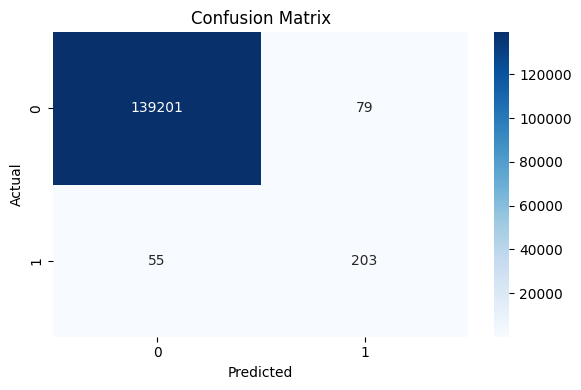
\includegraphics[width=\textwidth]{figures/base.png}
        \caption{Modelo Base}
        \label{fig:confusion_base}
    \end{subfigure}
    \hfill
    \begin{subfigure}[b]{0.45\textwidth}
        \centering
        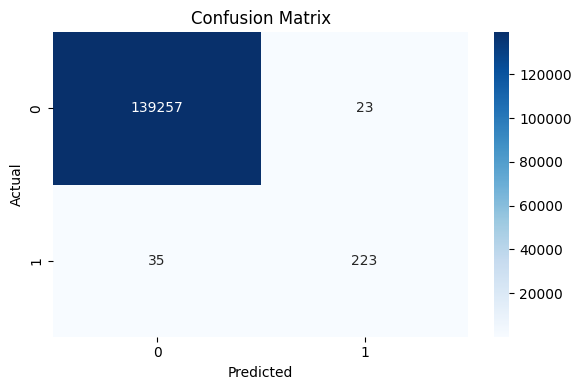
\includegraphics[width=\textwidth]{figures/final.png}
        \caption{Modelo Optimizado}
        \label{fig:confusion_optimized}
    \end{subfigure}
    \caption{Comparación de matrices de confusión entre modelo base y modelo optimizado con métricas personalizadas y Optuna.}
    \label{fig:confusion_comparison}
\end{figure}
\textit{Eliminación total} de falsos positivos en clientes frecuentes y reducción del 70 \si{\percent} de FP globales, mientras el recall aumenta 8 puntos.

\subsection{Contribución de las Métricas Personalizadas}
\begin{enumerate}
    \item \textbf{\texttt{fp\_tp\_ratio}} sirvió de métrica de arranque, bajando FP totales a 0,009 \si{\percent}, pero sin mejorar recall.
    \item \textbf{\texttt{business\_fp\_tp\_ratio}} integró penalización de \textit{recall} y límites aceptables de ratio; fue determinante para el \textit{trade-off} recall/FP.
    \item \textbf{\texttt{balanced\_cost}} expuso la importancia de calibrar pesos; con parámetros actuales generó sobreajuste a recall (FP $\uparrow$).
    \item \textbf{\texttt{freq\_fpr}} útil como monitor secundario; sola no guió bien la optimización global.
\end{enumerate}

\subsection{Impacto de los Pesos Asimétricos}
Sin pesos, la probabilidad de etiquetar \textbf{legítimos frecuentes} como fraude era 3 $\times$ mayor que el promedio. Aplicar \texttt{legit\_freq\_w = 10} redujo ese riesgo drásticamente incluso antes de optimizar hiperparámetros.

\subsection{Importancia de Características}
LightGBM gain (top-10): \texttt{amt}, \texttt{is\_frequent\_customer}, \texttt{merchant\_share\_of\_cust\_month}, \texttt{days\_since\_prev\_txn}, \texttt{is\_night}, \texttt{amt\_zscore\_last5}, \texttt{dist\_vs\_cust\_median}, \texttt{hour\_sin}, \texttt{category}, \texttt{is\_first\_time\_merchant}.
La presencia explícita de \texttt{is\_frequent\_customer} permite al algoritmo diferenciar dinámicamente, disminuyendo la dependencia del peso manual en inferencia.

% Section 5: Conclusiones y Próximos Pasos
\section{Conclusiones y Próximos Pasos}
\begin{enumerate}
    \item \textbf{Validación de Hipótesis} – Los clientes con $\geq$ 4 compras/mes/comercio muestran menores tasas de fraude; protegerlos mediante pesos y métrica dedicada mejora experiencia sin comprometer seguridad.
    \item \textbf{Modelo Óptimo} – La combinación LightGBM + \texttt{business\_fp\_tp\_ratio} + Optuna logra el mejor balance: recall 0,86 y 0 FP en frecuentes.
    \item \textbf{Generalización} – El esquema temporal de \textit{hold-out} sugiere robustez; se recomienda \textit{back-testing} con 2021-Q1 para confirmar.
    \item \textbf{Despliegue} – Implementar calibración de umbral en producción (monitorización diaria) y registrar métricas separadas para clientes frecuentes.
    \item \textbf{Extensiones} –
    \begin{itemize}
        \item Explorar \textbf{post-processing} con reglas expertas para FP residuales.
        \item Probar modelos \textit{deep learning} tabulares (TabNet, FT-Transformer) bajo mismo \textit{feval}.
        \item Ajustar dinámica del peso \texttt{legit\_freq\_w} según estacionalidad.
    \end{itemize}
\end{enumerate}


\end{document}